\documentclass[tikz,border=10pt]{standalone}
\usepackage{tikz}
\usetikzlibrary{arrows.meta,positioning,calc}

\begin{document}
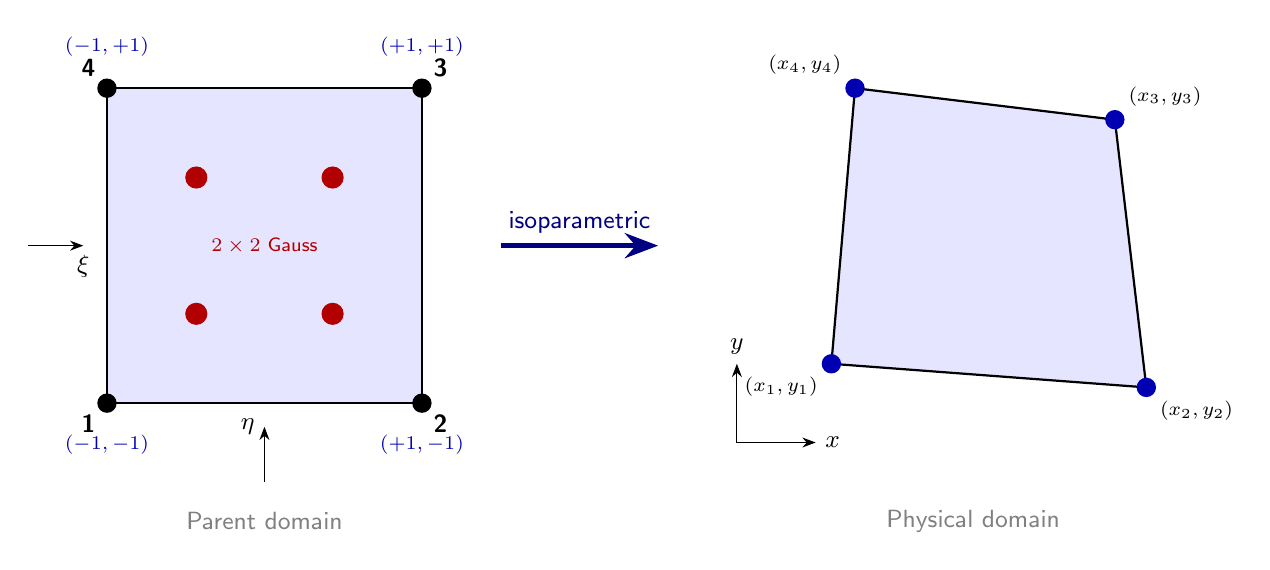
\begin{tikzpicture}[
    node font=\sffamily,
    >=Stealth,
    node dot/.style={circle, fill=black, inner sep=0pt, minimum size=7pt},
    node hollow/.style={circle, draw=black, fill=white, inner sep=0pt, minimum size=7pt, line width=1pt},
]

% === LEFT: Parent Domain ===
\begin{scope}
    % Square fill
    \fill[blue!10] (-2,-2) rectangle (2,2);
    \draw[thick] (-2,-2) rectangle (2,2);
    
    % Gauss points
    \foreach \x/\y in {-0.577/-0.577, 0.577/-0.577, 0.577/0.577, -0.577/0.577} {
        \fill[red!70!black] (\x*1.5,\y*1.5) circle (4pt);
    }
    
    % Nodes
    \node[node dot] (p1) at (-2,-2) {};
    \node[node dot] (p2) at (2,-2) {};
    \node[node dot] (p3) at (2,2) {};
    \node[node dot] (p4) at (-2,2) {};
    
    % Node labels
    \node[below left=1pt, font=\small\bfseries] at (p1) {1};
    \node[below right=1pt, font=\small\bfseries] at (p2) {2};
    \node[above right=1pt, font=\small\bfseries] at (p3) {3};
    \node[above left=1pt, font=\small\bfseries] at (p4) {4};
    
    % Natural coordinates
    \node[below=8pt, font=\scriptsize, blue!70!black] at (p1) {$(-1,-1)$};
    \node[below=8pt, font=\scriptsize, blue!70!black] at (p2) {$(+1,-1)$};
    \node[above=8pt, font=\scriptsize, blue!70!black] at (p3) {$(+1,+1)$};
    \node[above=8pt, font=\scriptsize, blue!70!black] at (p4) {$(-1,+1)$};
    
    % Axes
    \draw[->] (0,-3) -- (0,-2.3) node[left, font=\small\itshape] {$\eta$};
    \draw[->] (-3,0) -- (-2.3,0) node[below, font=\small\itshape] {$\xi$};
    
    % Label
    \node[font=\small, gray] at (0,-3.5) {Parent domain};
    
    % 2x2 Gauss label
    \node[font=\scriptsize, red!70!black] at (0,0) {$2\times2$ Gauss};
\end{scope}

% === ARROW ===
\draw[->, very thick, blue!50!black, line width=2pt] (3,0) -- (5,0) 
    node[midway, above, font=\small] {isoparametric};

% === RIGHT: Physical Domain ===
\begin{scope}[xshift=9cm]
    % Distorted quad
    \fill[blue!10] (-1.8,-1.5) -- (2.2,-1.8) -- (1.8,1.6) -- (-1.5,2) -- cycle;
    \draw[thick] (-1.8,-1.5) -- (2.2,-1.8) -- (1.8,1.6) -- (-1.5,2) -- cycle;
    
    % Nodes
    \node[node dot, fill=blue!70!black] (q1) at (-1.8,-1.5) {};
    \node[node dot, fill=blue!70!black] (q2) at (2.2,-1.8) {};
    \node[node dot, fill=blue!70!black] (q3) at (1.8,1.6) {};
    \node[node dot, fill=blue!70!black] (q4) at (-1.5,2) {};
    
    % Coordinate labels
    \node[below left=2pt, font=\scriptsize\itshape] at (q1) {$(x_1,y_1)$};
    \node[below right=2pt, font=\scriptsize\itshape] at (q2) {$(x_2,y_2)$};
    \node[above right=2pt, font=\scriptsize\itshape] at (q3) {$(x_3,y_3)$};
    \node[above left=2pt, font=\scriptsize\itshape] at (q4) {$(x_4,y_4)$};
    
    % Axes
    \draw[->] (-3,-2.5) -- (-2,-2.5) node[right, font=\small\itshape] {$x$};
    \draw[->] (-3,-2.5) -- (-3,-1.5) node[above, font=\small\itshape] {$y$};
    
    % Label
    \node[font=\small, gray] at (0,-3.5) {Physical domain};
\end{scope}

\end{tikzpicture}
\end{document}
